\section{Introduction}
\label{sec:introduction}

Software systems undergo many changes during their lifetime, and often
such changes can adversely affect the software. 
To avoid undesirable changes or unexpected bugs, software engineers need to  
test the overall functionality of the system before deploying a new release 
of the product. One of the common ways to evaluate system quality 
in a sequence of releases is regression testing.
In regression testing, software engineers validate the software system
to ensure that new changes have not introduced new faults or that they don't 
affect the other parts of the system. However, modern software systems 
evolve frequently, and their size and complexity grow quickly, and thus  
the cost of regression testing can become too expensive~\cite{jeff16}. 
To reduce regression testing cost, many regression testing and maintenance
approaches including test selection and test prioritization~\cite{marksurvey}.

To date, the majority of regression testing techniques have utilized various 
software metrics that are available from software repositories, such as
the size and complexity of the application, code coverage, fault history information, 
and dependency relations among components. 
Further, various empirical studies have shown that the use of a certain metric or 
a combination of multiple metrics can improve the effectiveness of
regression testing techniques better than other metrics. For example, Anderson et 
al.~\cite{jeff14} empirically investigated the use of various code features
mined from a large software repository, showing that these code features
can help improve regression testing processes.
However, we believe that, rather than simply picking one metric over another, 
adopting a recommender system, that identifies more relevant metrics by considering 
software characteristics and the software testing environment would provide a better solution.

Recommender systems have been utilized to help reduce the decision making 
effort by providing a list of relevant items to users based on a 
user's preference or item attributes.
For example, companies that produce daily-life applications, such as Netflix, 
Amazon, and many social networking applications~\cite{recomsurvey05}
are adopting recommender systems to provide more personalized services so that
they can attract more users. 
Recently, recommender systems have been used in software engineering areas 
to improve various software engineering tasks. 
For example, Mens et al. provide a source code recommendation 
system to help the developer by giving hint and suggestions or  
by correcting an existing code ~\cite{coderecommender}. 
Zanjani et al. performed a study by developing a recommender system for
code review based on historical contributions of prior reviews ~\cite{sara}. 
Anvik et al. conducted research that applied machine learning techniques
to developers and bug history to make suggestions about 
``who should fix this bug?''~\cite{who}.
While many software engineering techniques have started to incorporate 
recommendation systems, no researchers have investigated the use 
of recommender systems in the area of regression testing.

Therefore, we investigate whether the use of recommender systems can
help improve regression testing techniques, in particular focusing 
on test case prioritization.
In this paper, we propose an item-based collaborative filtering recommender 
system that uses the user interactions data
and application change history information.
We implemented a test case prioritization technique by applying our recommender system
and performed an empirical study using two open source software systems and one commercial system.
The results of our study show that our proposed recommender system approach can 
improve the effectiveness of test case prioritization 
compared to four other control techniques.
Further, our results indicate that our proposed approach yielded higher
scores than traditional prioritization techniques 
when companies have limited time budgets. 

\begin{figure*}[!hb]
        \centering
        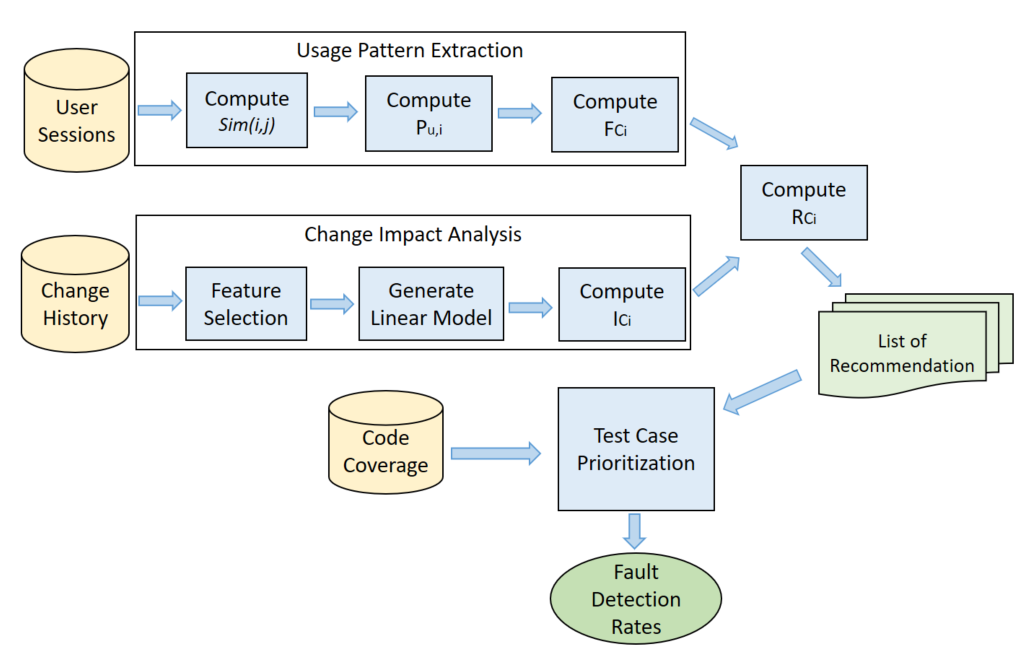
\includegraphics[width=0.75\linewidth]{./Overview6.png}
        \vspace*{3pt}
        \caption{An Overview of Our Test Case Recommender System}
        \label{fig:workflow}
\end{figure*}

The main contributions of this research are as follows:
(1) We proposed an item-based recommender system that improves test prioritization, 
(2) We performed empirical evaluations of the proposed technique and four other control techniques, and
(3) We provided guidance to testers and discussed practical considerations when
    they apply recommendation systems during testing.

The rest of the paper is organized as follows. In Section ~\ref{sec:approach}, we
discuss the approach used in this research and formally define
collaborative filtering recommender systems. 
Sections~\ref{sec:study} and \ref{sec:data} present our empirical study,
including design, results, and analysis.
Section~\ref{sec:discussion} discusses the results and the implications of these results. 
Section~\ref{sec:validity} discusses potential threats to validity and
Section~\ref{sec:related-work} presents background and related work. 
Finally, in Section~\ref{sec:conclusions}, 
we provide conclusions and discuss future work.

